% !TEX root = ../intro-stellar-physics.tex

\section{The luminosity equation}

We've established the relations for the enclosed mass,
\begin{equation}\label{e.mass}
\DD{m}{r} = 4\pi r^{2}\rho,
\end{equation}
the pressure,
\begin{equation}\label{e.pressure}
\DD{P}{r} = -\rho\frac{Gm}{r^{2}},
\end{equation}
and the temperature,
\begin{eqnarray}\label{e.temperature-radiative}
\DD{T}{r} &=& - \frac{L}{4\pi r^{2}}\frac{3\rho\kappa}{4ac T^{3}}\qquad \textrm{in radiative regions;} \\ 
\label{e.temperature-convective}
\DD{T}{r} &=& \frac{T}{P}\tderiv{\ln T}{\ln P}{S}\DD{P}{r} \quad \textrm{in convective regions}.
\end{eqnarray}
We need an equation for the luminosity $L(r)$, which we now derive.

\begin{marginfigure}
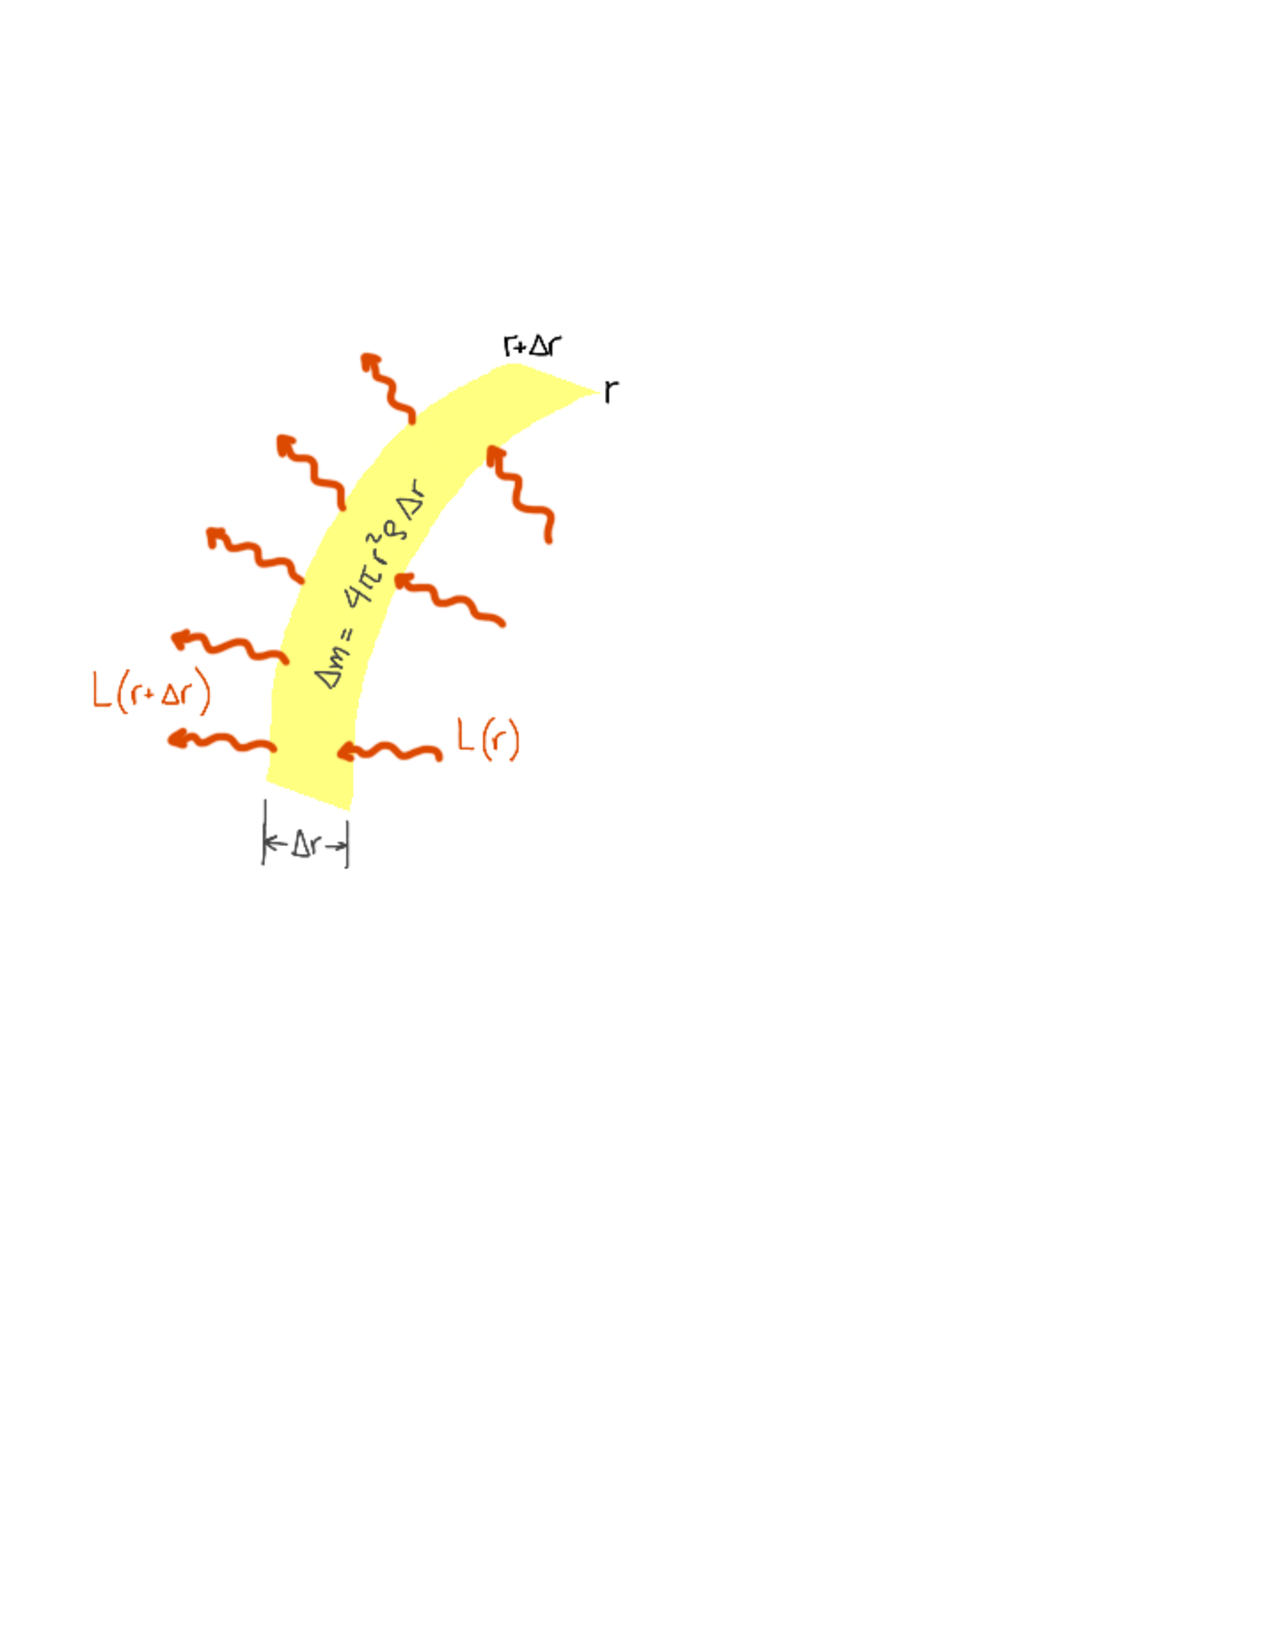
\includegraphics[width=\linewidth]{luminosity}
\caption[Heat balance in a mass shell]{Heat balance in a shell $\Delta m$.}
\label{f.luminosity}
\end{marginfigure}
Suppose we have a shell of mass $\Delta m$ lying between surfaces $r$ and $r+\Delta r$.  The shell gains heat from nuclear reactions at a rate $\Delta m \times \varepsilon$, where $\varepsilon$ is the heating rate per unit mass.  In addition, there is heat entering the shell from below at a rate $L(r)$ and heat leaving the top of the shell at a rate $-L(r+\Delta r)$.
If the shell is neither gaining or losing heat, then these terms must balance:
\[ 4\pi r^{2}\rho\varepsilon + L(r) - L(r+\Delta r) = 0. \]
This reduces to our fourth equation of stellar structure,
\begin{equation}
\label{e.luminosity}
\DD{L}{r} = 4\pi r^{2}\rho\varepsilon.
\end{equation}
These equations are supplemented by an equation of state $P = P(\rho,T)$.

\section{Burning stages of stellar evolution}

\subsection{Hydrogen burning via pp reactions: the lower main sequence}

In a contracting pre-main sequence star, the reaction $\hydrogen[2]+p\to\gamma+\helium[3]$ proceeds rapidly owing to the small Coulomb barrier; in fact, this reaction can occur in objects as small as $\approx \val{12}{M_{\mathrm{Jupiter}}}$.  The small primordial abundance of deuterium, however, prevents this reaction from doing anything more than slowing contraction slightly.  The reaction $\pt +\pt$ is much slower, because there is no bound nucleus \helium[2]; the only possible way to form a nucleus is to have a weak interaction as well, giving the reaction $\pt+\pt\to e^{+}+\nu_{e}+\hydrogen[2]$.

The weak cross section goes roughly as $\sigma_{\mathrm{weak}} \sim \val{10^{-20}}{\barn}\left(E/\keV\right)$, so that
\[ \frac{\sigma_{\mathrm{weak}}}{\sigma_{\mathrm{nuc}}} \sim 10^{-23}\left(\frac{E}{\keV}\right). \]
The $S$-factor for the $\pt+\pt$ reaction is very small, and as a result the characteristic temperature for this reaction to occur is $\approx \val{\sci{1.5}{7}}{\K}$; at this temperature, the lifetime of a proton to forming deuterium via capture of another proton is about $\val{6}{\Giga\yr}$.  Once a deuterium nucleus is formed, it is immediately destroyed via $\hydrogen[2]+p\to\gamma+\helium[3]$. The nucleus \lithium[4] is unbound with a lifetime of $\val{10^{-22}}{\second}$; the nucleus \beryllium[6] is likewise unbound ($\tau \sim \val{\sci{5}{-21}}{\second}$). As a result, the next reaction that can occur is $\helium[3]+\helium[3]\to 2\pt+\helium$.  Despite having a much greater Gamow energy than $\pt + \pt$, this reaction still is much faster than $\pt+\pt$ owing to the small weak cross-section.

In addition to capturing another \helium[3], it is also possible that
\begin{eqnarray}
\helium[3] + \helium &\to& \beryllium[7] + \gamma\nonumber\\
 \beryllium[7] + e^{-} &\to& \lithium[7] +  \nu_{e}\qquad(\tau=\val{53}{\unitstyle{d}})\nonumber \\
 \lithium[7] + \pt &\to& 2\helium + \gamma;
 \end{eqnarray}
furthermore, at slightly higher temperatures \beryllium[7] can capture a proton instead of an electron, giving the third branch
\begin{eqnarray}
\beryllium[7] + \pt &\to& \boron[8] + \gamma\nonumber\\
\boron[8] &\to& \beryllium[8] + e^{+} + \nu_{e}\qquad(\tau = \val{770}{\milli\second})\nonumber\\
\beryllium[8] &\to& 2\helium\qquad(\tau= \val{10^{-16}}{\second}).
\end{eqnarray}
 The end result of these chains is the conversion of hydrogen to helium, although the amount of energy carried away by neutrinos differs from one chain to the next.

\subsection[The CNO cycle]{Hydrogen burning via the CNO cycle: the upper main sequence}

As we saw in the previous section, the smallness of the $\pt+\pt$ cross-section means that captures onto heavier nuclei can be competitive at stellar temperatures.  Let's get a rough estimate of how charged a nucleus can be before the Coulomb barrier makes the reaction slower than $\pt+\pt$.  Assuming $A = 2Z$, and taking the $S$-factor for $\pt+\pt$ to be $10^{-22}$ times smaller that that for $\pt + \mathrm{^{A}Z}$ gives us the rough equation
\[ 10^{-22}\exp\left(-\frac{33.81}{T_{6}^{1/3}}\right) \approx \exp\left(-\frac{41.47 Z^{2/3}}{T_{6}^{1/3}}\right), \]
where the factors in the exponentials come from the peak energy for the reaction (see the handout on nuclear burning), and $T_{6}\equiv (T/\val{10^{6}}{\K})$.  Solving for $Z$, we see that at $T_{6} = 10$, proton captures onto \carbon\ have a comparable cross-section to $\pt + \pt$; at $T_{6} = 20$, proton captures onto \oxygen\ have a comparable cross-section.

Thus at temperatures slightly greater than that in the solar center, the following catalytic cycle becomes possible.
\begin{center}
\begin{tabular}{rr}
reaction & $\log[(\tau/\yr) \times (\rho X_{H}/\val{100}{\grampercc})]$\\
\hline
$\carbon(\mathbf{p},\gamma)\nitrogen[13]$ & 3.82\\
$\nitrogen[13](,e^{+}\nu_{e})\carbon[13]$ & $\tau=\val{870}{\second}$\\
$\carbon[13](\mathbf{p},\gamma)\nitrogen[14]$ & 3.21\\
$\nitrogen[14](\mathbf{p},\gamma)\oxygen[15]$ & 5.89 \\
$\oxygen[15](,e^{+}\nu_{e})\nitrogen[15]$ & $\tau = \val{178}{\second}$\\
$\nitrogen[15](\mathbf{p},\mathbf{^4He})\carbon$ & 1.50 \\
\hline
\end{tabular}
\end{center}
As indicated by the boldfaced symbols, this cycle takes in 4 protons and releases 1 helium nucleus.
The reaction timescales are evaluated at a temperature of $\val{20}{\Mega\K}$.
The reaction $\nitrogen+\pt\to\gamma+\oxygen[15]$ is by far the slowest step in the cycle; as a result, all of the CNO elements are quickly converted into \nitrogen\ in the stellar core, and this reaction controls the rate of heating.  At $T = \val{\sci{2}{7}}{\K}$, $\dif \ln \varepsilon_{\mathrm{CNO}}/\dif\ln T = 18$; in contrast the $\pt+\pt$ reaction has a temperature exponent of only 4.5.

The strong temperature dependence of the CNO burning has two effects on the structure of the star.  First, it makes the central temperature nearly constant over a wide range of stellar masses for $M > \val{1}{\Msun}$. A constant central temperature implies, via the virial theorem, that $R \propto M$ on the upper main sequence.  A second consequence is that nearly all of the star's luminosity is generated in a small mass about the stellar center.  This drives the cores of massive stars to be convective.

\section{Summary}

This convective zone changes the structure of the star, so that $L\sim M^{3.5}$ rather than the $M^{3}$ scaling we derived earlier.  It also means the star can burn more of the hydrogen in its interior.  The hotter $\Teff$ means, however, that the opacity is less strong in the surface layers of upper main sequence stars, and so the outer layers are radiative.  Table~\ref{t.MS-characteristics} gives a summary of the properties of main sequence stars.
\begin{margintable}[-6\baselineskip]
\caption{\label{t.MS-characteristics} Characteristics of main-sequence stars}
\centering
\begin{tabular}{lll}
characteristic & $M\lesssim\Msun$ & $M\gtrsim\Msun$\\
\hline
hydrogen burning & pp & CNO\\
core & radiative  & convective\\
envelope & convective & radiative\\
\end{tabular}
\end{margintable}
